\documentclass[aspectratio=169,10pt]{beamer}
\usetheme{metropolis}
\usepackage{amsmath,amssymb,booktabs}
\usepackage{tikz}
\usetikzlibrary{positioning,arrows.meta}
\graphicspath{{../figures/}{./}}
\setbeamertemplate{navigation symbols}{}
\newcommand{\R}{\mathbb{R}}
\newcommand{\E}{\mathbb{E}}
\newcommand{\spk}{}
\setbeamertemplate{frame footer}{\spk}

\title{The Virtue of Complexity Everywhere}
\subtitle{Factor timing with random features: the paper and our equity replication}
\author{Team 1: Luwei Cai, Hongjun Ding, Yueqi Lin, Hao Li}
\institute{Deep Learning in Finance, Assignment 1\\Baruch MFE, Fall 2026}
\date{}

\begin{document}
\maketitle
\addtocounter{framenumber}{1}

% ================= Luwei: 1-3 =================
\renewcommand{\spk}{Presenter: Luwei Cai}
\begin{frame}{The question: can a huge model forecast with little data?}
\textbf{Financial question.} Can we time US equity factors out of sample?
\begin{itemize}
  \item Returns are noisy, histories are short (the paper's key case: $T=12$ months)
  \item Textbook (Occam): few parameters, $L\ll T$, otherwise you fit noise
\end{itemize}
\vspace{4pt}
\textbf{Lecture view (Part III).} No return model is correctly specified.
\begin{itemize}
  \item \emph{Correctly specified:} complexity is a pure statistical cost (double descent)
  \item \emph{Misspecified} (returns): richer models remove approximation error; with shrinkage that gain can outrun the added noise
\end{itemize}
\vspace{4pt}
\textbf{Paper (Kelly--Malamud--Zhou 2022):} take $L\gg T$ and test it on 159 equity factors.\\
\alert{A conditional claim:} Sharpe rises with complexity \emph{when ridge shrinkage is large enough}.
\end{frame}

\begin{frame}{Setup and notation (as in the paper)}
\begin{tabular}{@{}ll@{}}
$X_t\in\R^{d}$ & raw signals at $t$: $d=15$ (Welch--Goyal) or $d=2$ (momentum) \\
$R_{t+1}$ & next-month factor return, scaled by ex-ante volatility \\
$S_t\in\R^{L}$ & the $L$ random features used, built from $X_t$ \\
$P=7p$ & random weights $\omega_i$ per draw ($p$ per bandwidth); each gives a sin and a cos feature \\
$T$ & months in the rolling training window ($12,\,60,\,120$) \\
$c=L/T$ & complexity; $c=1$ is the interpolation boundary \\
$z$ & ridge penalty ($10^{-3}$ to $10^{3}$) \\
$\hat\beta_t$ & the only learned weights ($L$ of them) \\
\end{tabular}
\vspace{6pt}
\begin{itemize}
  \item Raising $L$ adds transformations of the \emph{same} $d$ signals, not new data
  \item \textbf{Two separate studies, 159 factors, one model per factor:} A = 15 Welch--Goyal signals; B = 2 momentum signals (current month, prior 11-month mean). Never combined.
\end{itemize}
\end{frame}

\begin{frame}{What each factor series looks like}
\begin{itemize}
  \item \textbf{Universe:} 6 French-library factors + 153 JKP characteristic factors, monthly
  \item \textbf{Equities only here:} the paper also uses 44 futures and Treasuries; we do not
  \item \textbf{Scaling, past data only:} returns by trailing 12-month RMS; signals by expanding RMS (at least 36 months), clipped to $[-5,5]$
  \item \textbf{Target and evaluation:} out-of-sample, rolling window; metrics averaged over 100 feature draws, then over factors
\end{itemize}
\vspace{6pt}
\textbf{Data check.} Our recomputed annualised mean, volatility and Sharpe correlate $0.996$, $0.9995$, $0.997$ with the paper's Table 1 (158 matched factors).
\end{frame}

% ================= Hongjun: 4-6 =================
\renewcommand{\spk}{Presenter: Hongjun Ding}
\begin{frame}{Model: fixed random features, learned ridge weights}
\centering
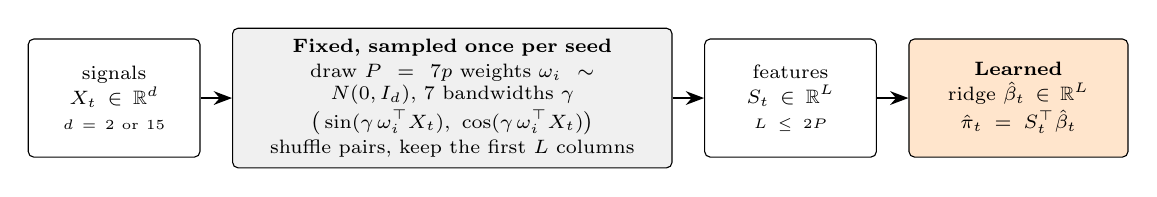
\begin{tikzpicture}[font=\scriptsize,
  box/.style={draw,rounded corners=2pt,align=center,inner sep=4pt,minimum height=1.5cm},
  fix/.style={box,fill=black!6},
  lrn/.style={box,fill=orange!20},
  arr/.style={-{Stealth},thick}]
\node[box,text width=1.9cm] (g) {signals\\[1pt]$X_t\in\R^{d}$\\[1pt]{\tiny $d=2$ or $15$}};
\node[fix,text width=5.3cm,right=0.4cm of g] (f) {\textbf{Fixed, sampled once per seed}\\[1pt]
 draw $P=7p$ weights $\omega_i\sim N(0,I_d)$, 7 bandwidths $\gamma$\\[1pt]
 $\big(\sin(\gamma\,\omega_i^\top X_t),\ \cos(\gamma\,\omega_i^\top X_t)\big)$\\[1pt]
 shuffle pairs, keep the first $L$ columns};
\node[box,text width=1.9cm,right=0.4cm of f] (s) {features\\[1pt]$S_t\in\R^{L}$\\[1pt]{\tiny $L\le 2P$}};
\node[lrn,text width=2.5cm,right=0.4cm of s] (b) {\textbf{Learned}\\[1pt]ridge $\hat\beta_t\in\R^{L}$\\[1pt]$\hat\pi_t=S_t^\top\hat\beta_t$};
\draw[arr] (g)--(f); \draw[arr] (f)--(s); \draw[arr] (s)--(b);
\end{tikzpicture}

{\scriptsize Same $\omega$ for every factor at a given seed; 100 seeds; metrics averaged over seeds, then over the 159 factors}

\vspace{4pt}
\raggedright
\textbf{Learned: ridge on the last $T$ months.}
\[
\hat\beta_t(z)=\Big(zI+\tfrac1T\sum_{\tau=t-T}^{t-1}S_\tau S_\tau^\top\Big)^{-1}\tfrac1T\sum_{\tau=t-T}^{t-1}S_\tau R_{\tau+1}
\ \Longleftrightarrow\ \min_\beta\ \tfrac1T\sum_\tau (R_{\tau+1}-\beta^\top S_\tau)^2+z\|\beta\|^2
\]
\begin{itemize}
  \item Nonlinear in $X_t$, linear in $\hat\beta$: a two-layer network with a frozen random first layer
  \item Loss is squared error. \alert{Sharpe is not optimised}; it is only evaluated
\end{itemize}
\end{frame}

\begin{frame}{Timing strategy and what we measure}
\centering
\begin{tabular}{cc}
\textbf{1. Forecast = position} & \textbf{2. Strategy return}\\[2pt]
$\hat\pi_t=S_t^\top\hat\beta_t$ & $\hat R_{t+1}=\hat\pi_t\,R_{t+1}$
\end{tabular}

\vspace{8pt}
\raggedright
\begin{itemize}
  \item \textbf{Timeline:} train on pairs up to $t$ (returns already realised), forecast at $t$, earn at $t+1$. No look-ahead
  \item \textbf{Metrics:} out-of-sample $R^2$, $\|\hat\beta\|$, expected return, volatility, annualised Sharpe of $\hat R$
  \item \textbf{Aggregation:} Sharpe per seed per factor, averaged over seeds, then over factors (not the Sharpe of a 159-factor portfolio)
  \item \textbf{Scale:} multiplying $\hat\beta$ by a positive constant changes $R^2$ and $\|\hat\beta\|$, but not Sharpe
\end{itemize}
\end{frame}

\begin{frame}{Why can $L\gg T$ work?}
\begin{itemize}
  \item At $c=1$ with tiny $z$ the model interpolates the sample: $\|\hat\beta\|$ and volatility spike, $R^2$ crashes (\textbf{double descent})
  \item For $c>1$ the ridge (minimum-norm) solution gets smoother and $\|\hat\beta\|$ falls
  \item As $c\to\infty$ the random-feature model approaches \textbf{kernel ridge regression}
  \item Implication: ``more complex'' means ``a better-behaved smoother of the same signals'', not ``more overfit''
\end{itemize}
\vspace{6pt}
\textbf{Paper's prediction at $T=12$:} low $z$: a dip near $c=1$, then recovery; large $z$: Sharpe increasing in $c$.\\[4pt]
\textbf{Caveat the lecture also stresses:} not a licence to add junk predictors.
\end{frame}

% ================= Yueqi: 7-9 =================
\renewcommand{\spk}{Presenter: Yueqi Lin}
\begin{frame}{Our implementation (equities only)}
\begin{itemize}
  \item Written from the paper's equations: features (36--37), rolling ridge in dual $T\times T$ form (so $L=7{,}000$ is cheap), metrics (41--51)
  \item Same 159 factors and same two signal sets (A, B)
  \item $T=12$: 100 feature draws; $T=60,120$: 10 draws
  \item \textbf{Cuts:} $L\le7{,}000$ (paper 12{,}000); futures and bonds not replicated (paid data)
  \item \textbf{Beyond the paper:} baselines, time-shuffled placebo, exact-kernel check, simulator
\end{itemize}
\end{frame}

\begin{frame}{Sharpe vs.\ complexity at $T=12$: paper (top) and ours (bottom)}
\centering
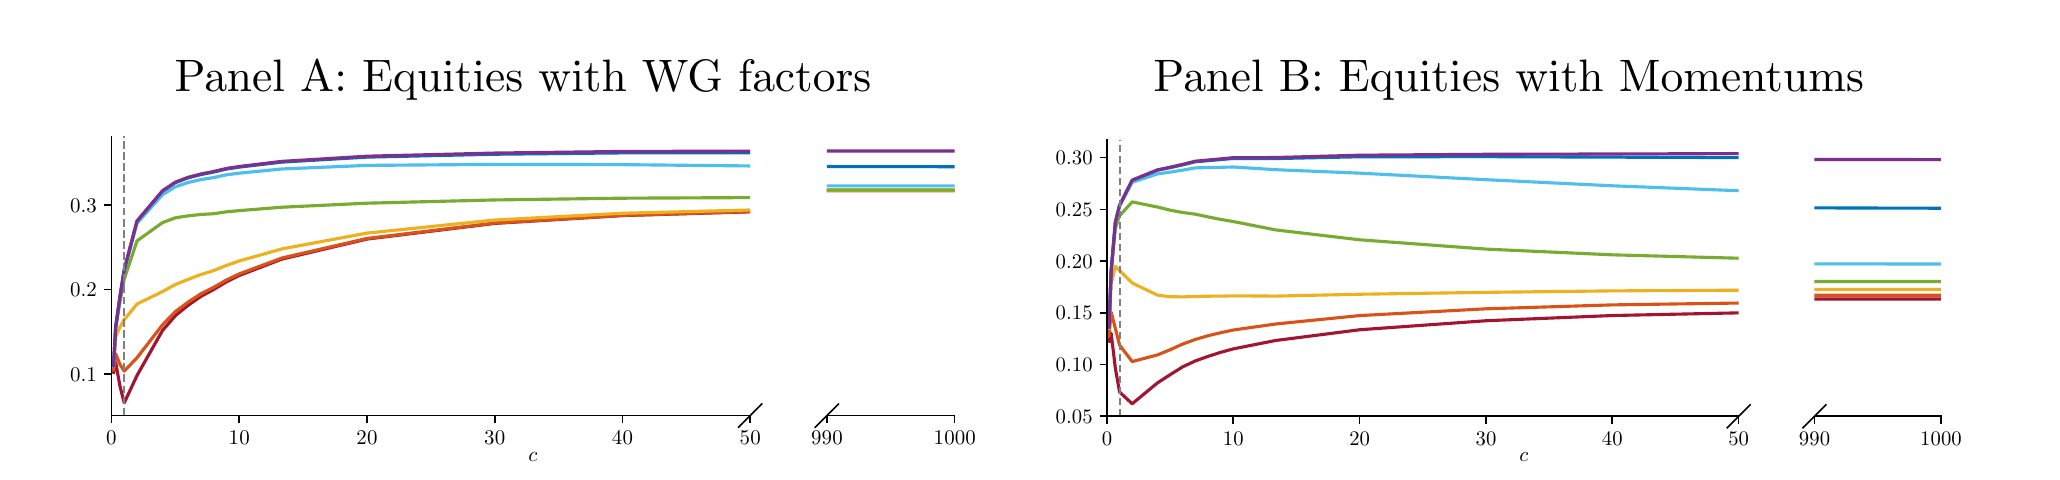
\includegraphics[width=0.74\textwidth]{paper_fig3.png}\hspace{4pt}\raisebox{0.2em}{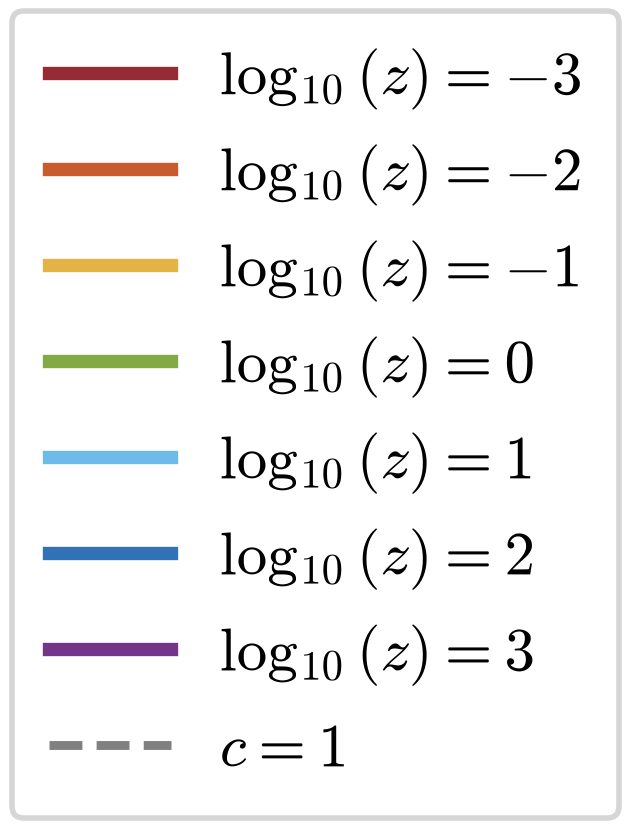
\includegraphics[height=0.2\textheight]{paper_legend.png}}\\[-1pt]
{\scriptsize Paper Fig.\ 3, panels A (Welch--Goyal) and B (momentum); broken $c$ axis. Same colour code in both rows}\\[3pt]
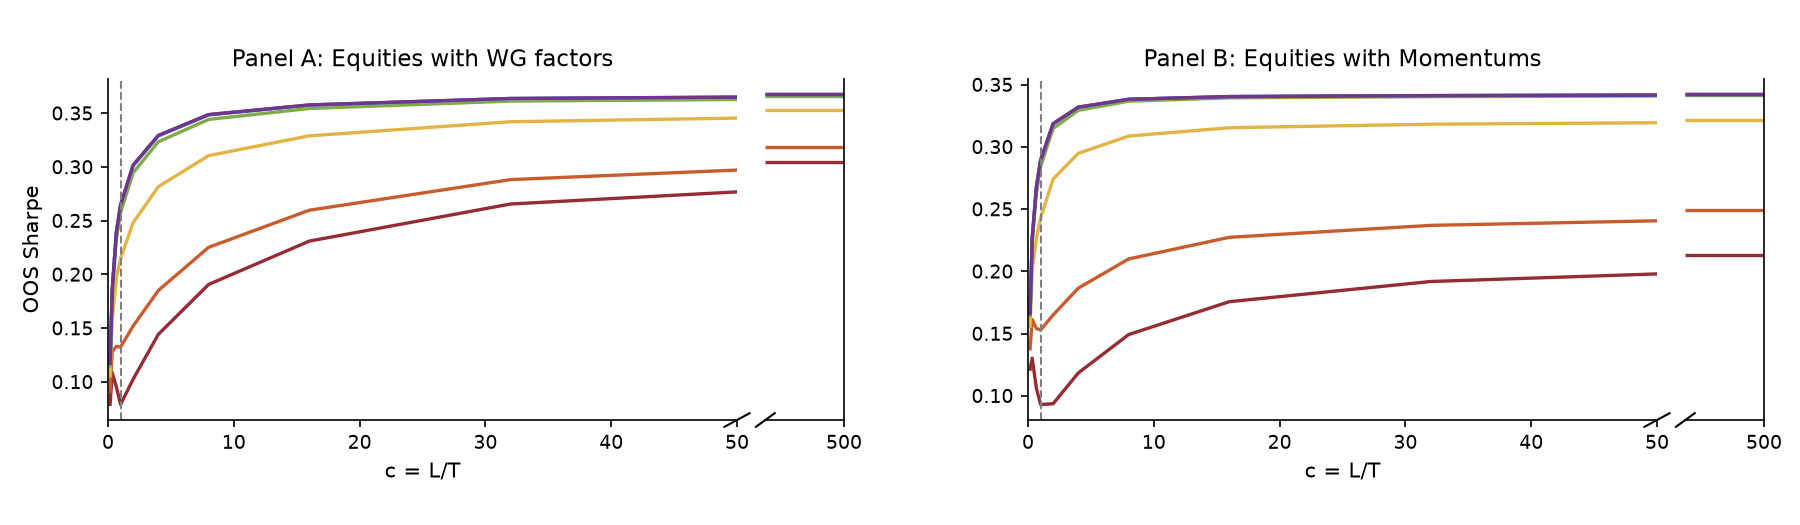
\includegraphics[width=0.8\textwidth]{fig3_T12_paperaxes.png}\\[-1pt]
{\scriptsize Ours: mean OOS Sharpe over 159 factors, same axes (linear $c$ to 50, break, largest model $c=500$ at right; paper 1{,}000)}
\end{frame}

\begin{frame}{Replication: close at $T=12$, weaker at longer $T$}
\centering
\begin{tabular}{lcccc}
\toprule
Mean Sharpe, large $z$ & $T=12$ ours & $T=12$ paper & $T=60$ & $T=120$ \\
\midrule
A: Welch--Goyal & 0.117 $\to$ 0.368 & $\approx$0.11 $\to$ 0.36 & +0.069 & +0.030 \\
B: Momentum & 0.166 $\to$ 0.342 & $\approx$0.10 $\to$ 0.30 & +0.068 & +0.018 \\
\bottomrule
\end{tabular}

{\footnotesize $T=12$: $c_{\min}\to c_{\max}$; $T=60,120$: rise. Paper values read off the figure by eye.}

\vspace{2pt}
\raggedright\small
\begin{itemize}
  \item \textbf{Sharpe (Fig.\ 3):} 96--98\% of factors improve; small $z$: dip at $c=1$ (0.093 vs paper $\approx$0.07), then recovery
  \item \textbf{$R^2$ (Fig.\ 1):} collapses near $c=1$ ($-1.67$) while Sharpe stays positive; $-0.18$ at $c=500$ (paper $\approx-0.45$)
  \item \textbf{Return, volatility (Fig.\ 2):} expected return matches at low $z$ (0.039 vs $\approx$0.04); volatility is lower (0.63 vs $\approx$0.8--0.9)
  \item \textbf{Longer windows (Fig.\ 5):} same direction, much smaller gain; Sharpe falls at $T=120$, $z=10^{-3}$
  \item \textbf{Not matched:} $\|\hat\beta\|$ plateaus (paper: falls); $z\ge1$ curves coincide (paper: fan out)
\end{itemize}
\end{frame}

\begin{frame}{Feature scaling: we use $1/\sqrt{L}$ (our main runs)}
\centering
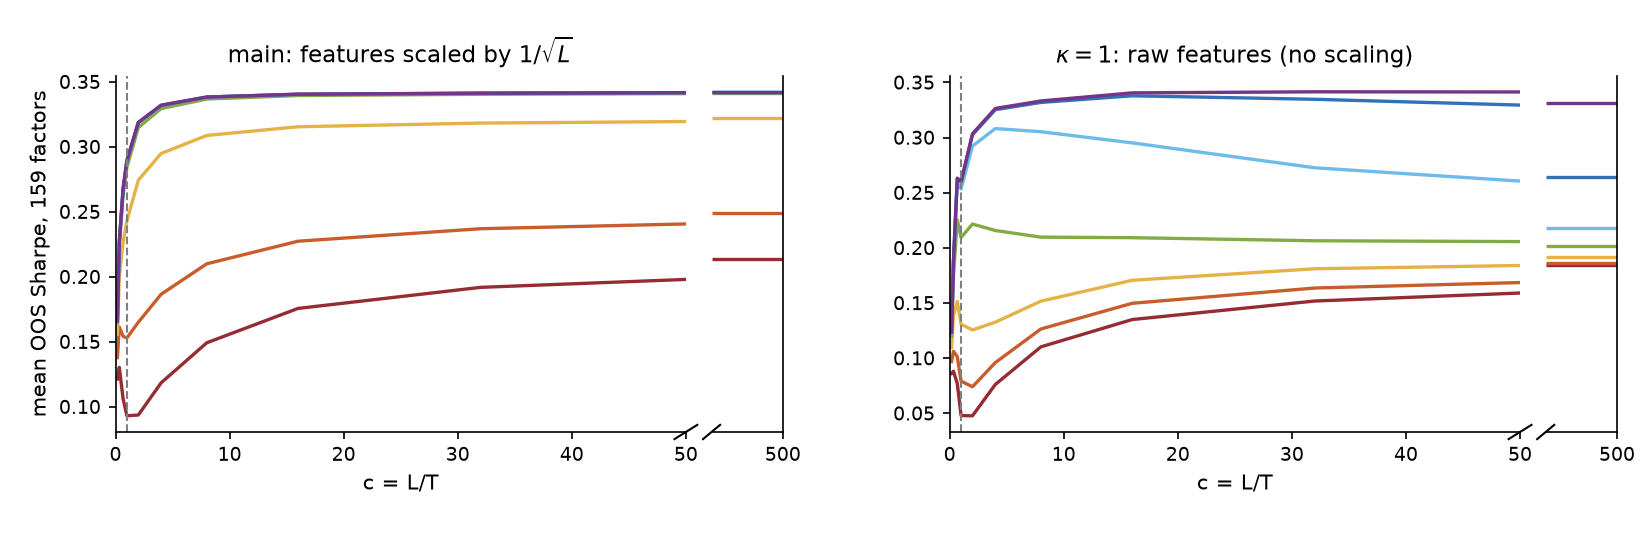
\includegraphics[width=0.68\textwidth]{scaling_slide.png}\\[-2pt]
{\scriptsize Ours, $T=12$, momentum. Left: main, $1/\sqrt{L}$: the kernel-consistent scaling (Rahimi--Recht; Sutherland--Schneider). Right: raw features ($\kappa=1$), a check with 10 draws}
\vspace{2pt}

{\scriptsize
\begin{tabular}{lccccccc}
\toprule
Sharpe at $c=500$ ($c=1000$ paper) & $z{=}10^3$ & $10^2$ & $10^1$ & $1$ & $10^{-1}$ & $10^{-2}$ & $10^{-3}$ \\
\midrule
Paper (by eye) & 0.30 & 0.25 & 0.20 & 0.17 & 0.17 & 0.16 & 0.15 \\
Ours, main ($1/\sqrt L$) & 0.342 & 0.342 & 0.342 & 0.342 & 0.322 & 0.249 & 0.213 \\
Ours, raw ($\kappa=1$) & 0.331 & 0.264 & 0.218 & 0.202 & 0.192 & 0.186 & 0.184 \\
\bottomrule
\end{tabular}}

\vspace{2pt}

{\scriptsize The paper does not state its scaling, so raw features are only a candidate. Best Sharpe is $\approx0.342$ under every scaling: our conclusions do not depend on it.}
\end{frame}

\begin{frame}{Beyond the paper: is the baseline fair?}
\centering
\begin{tabular}{lccc}
\toprule
Mean Sharpe, 159 factors (B) & $T=12$ & $T=60$ & $T=120$ \\
\midrule
Model, large $z$, $c_{\max}$ & 0.342 & 0.345 & 0.363 \\
Always long the vol-scaled factor & \textbf{0.353} & \textbf{0.354} & 0.351 \\
Trailing $T$-month mean & 0.338 & 0.309 & 0.303 \\
Linear ridge on same signals & 0.11--0.16 & 0.24--0.27 & 0.31--0.35 \\
\bottomrule
\end{tabular}
\vspace{6pt}
\raggedright
\begin{itemize}
  \item The paper's panels compare model sizes only: \textbf{no always-long benchmark}
  \item Model beats linear and trailing mean; it \textbf{ties} always-long ($T=12$: $-0.011$, s.e.\ 0.017)
  \item Always-long is flattering: factors are signed using the published findings
\end{itemize}
\end{frame}

\begin{frame}{Beyond the paper: placebo with time-shuffled signals}
\centering
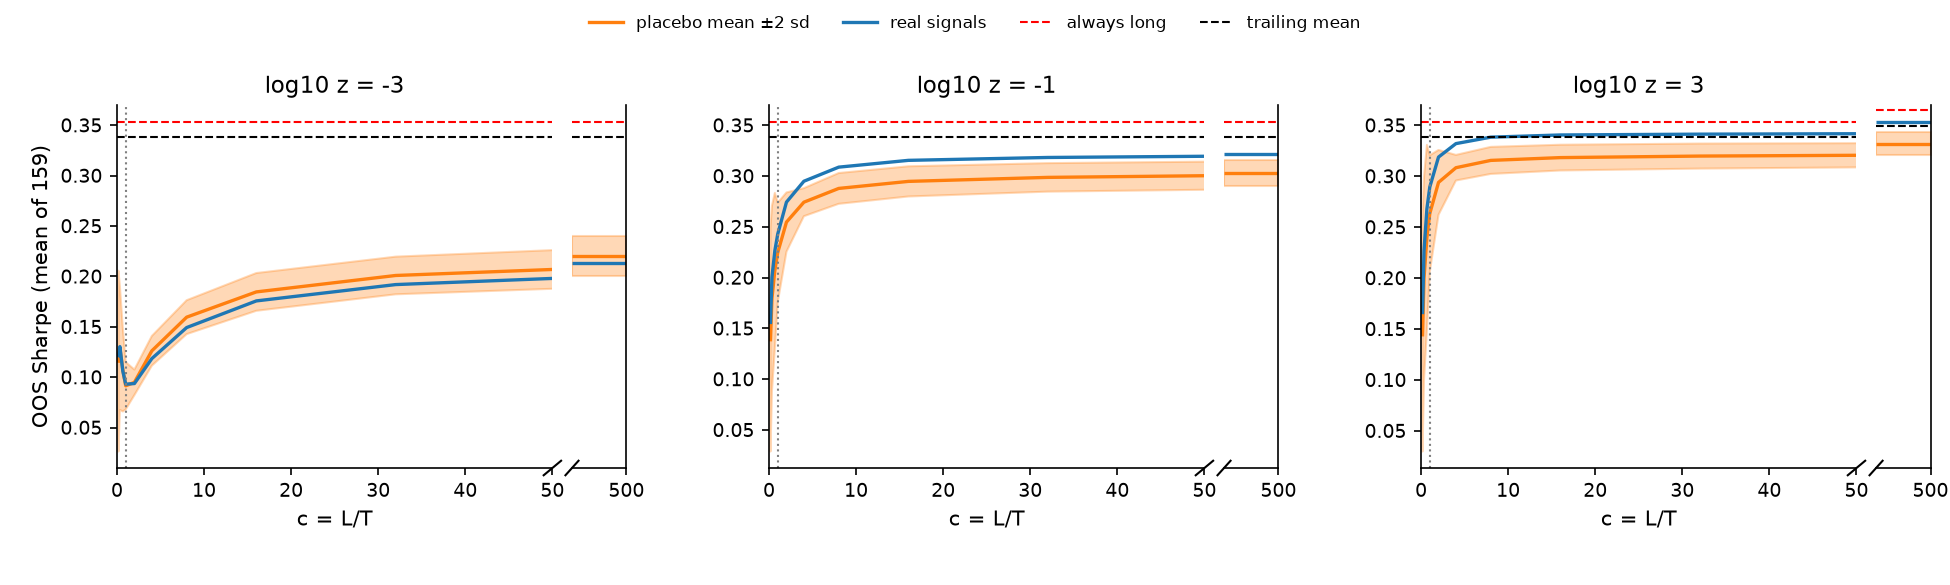
\includegraphics[width=0.97\textwidth]{placebo_paperaxes.png}
\vspace{-2pt}
\begin{itemize}\small
  \item Same rise with shuffled signals: $+0.177$ placebo vs $+0.176$ real ($z=10^3$, $T=12$)
  \item Real signals add about $+0.02$ (about 4 placebo s.d.) at high $c$; more at longer $T$ (+0.05 at 60, +0.07 at 120)
\end{itemize}
\end{frame}

% ================= Hao =================
\renewcommand{\spk}{Presenter: Hao Li}
\begin{frame}{Critique}
\begin{enumerate}
  \item \textbf{Mostly shrinkage.} The rise with $c$ is largely features converging to a kernel; learned predictability is a small part
  \item \textbf{Baseline.} Complexity levels are compared with each other, not with always-long
  \item \textbf{Hindsight} in factor selection and signs
  \item \textbf{No transaction costs} on a monthly-refit nonlinear position
  \item \textbf{Specification ambiguity:} the paper does not state its feature scaling or which kernel (eq.\ 36 vs 37); this moves the $z$ axis
  \item \textbf{Data:} 2022 paper vs.\ our 2026 data vintage
\end{enumerate}
\end{frame}

\begin{frame}{Takeaways}
\begin{itemize}
  \item \textbf{Replicated:} on 159 equity factors at $T=12$, Sharpe rises with $c$ (2--3$\times$), with a double-descent dip at small $z$
  \item \textbf{Qualified:} the gain fades at $T=60,120$ and needs large ridge
  \item \textbf{Not shown:} that complexity beats simply holding the factor, or that the rise is learned timing
  \item \textbf{Lesson:} the shape of the curve is robust; its economic value is not established
\end{itemize}
\vspace{8pt}
\centering\small Code, data and every number: \texttt{github.com/liny-r/Virtue-of-Complexity}
\end{frame}

% ================= Backup =================
\appendix
\renewcommand{\spk}{Presenter: Yueqi Lin}
\begin{frame}{Backup A: $R^2$ and $\|\hat\beta\|$ ($T=12$, ours)}
\centering
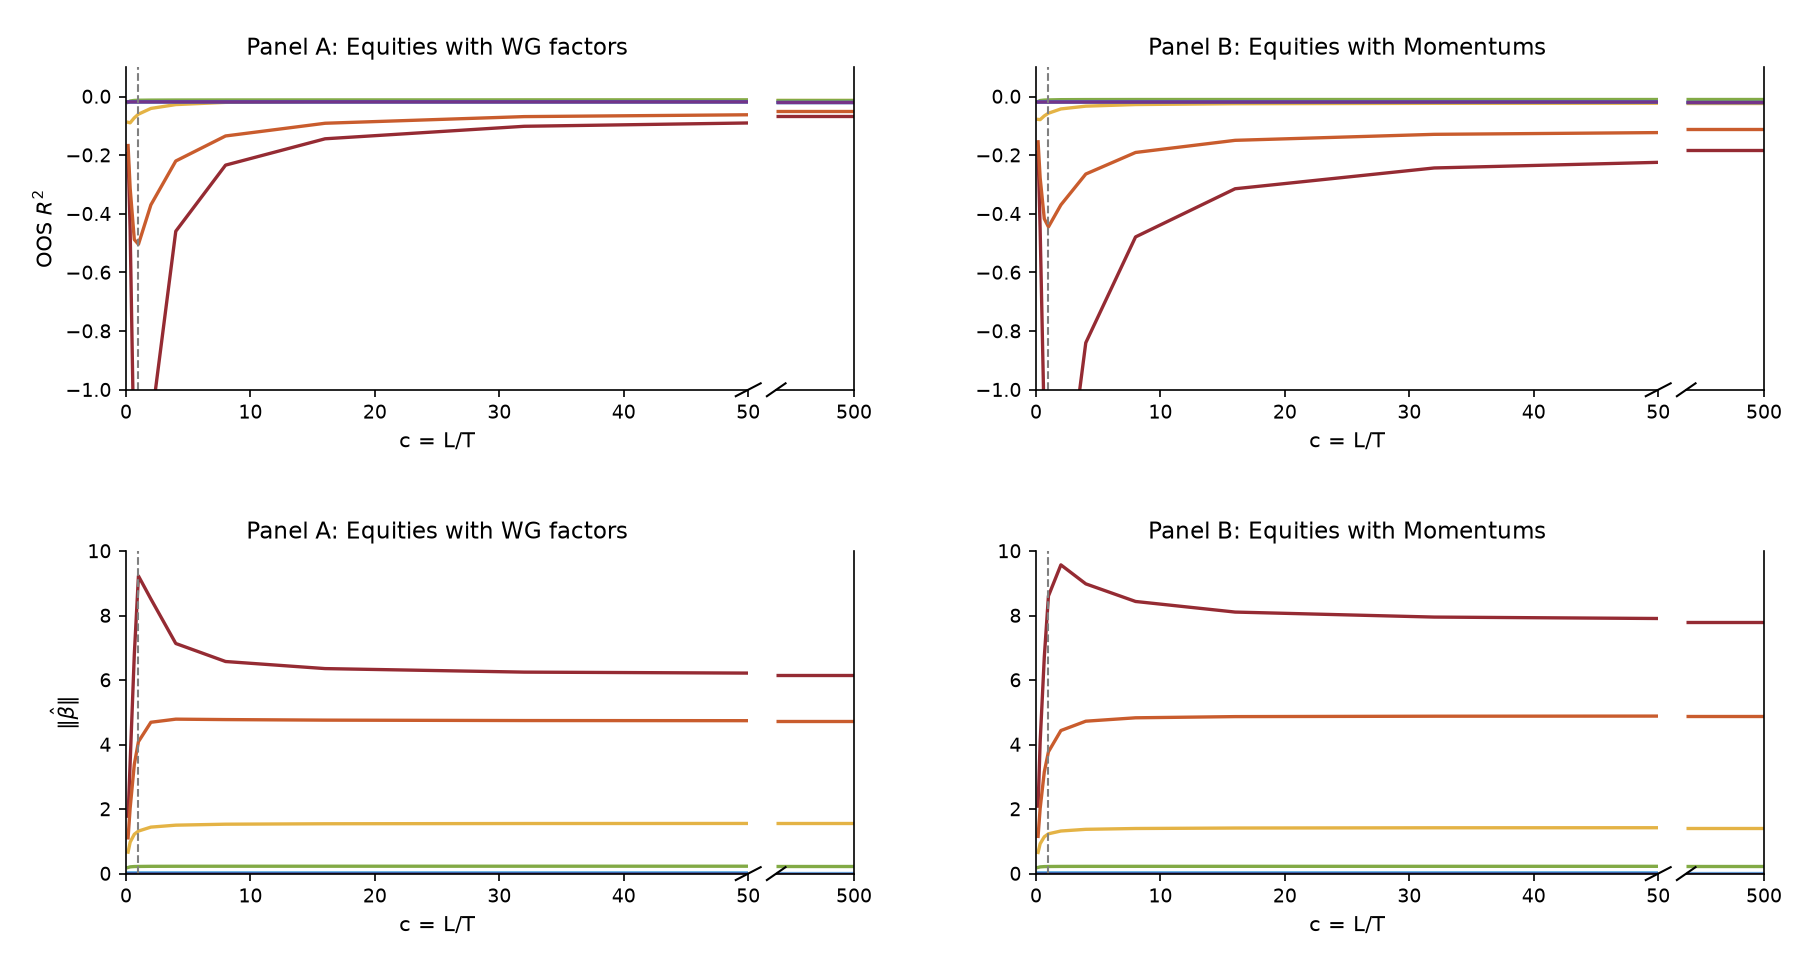
\includegraphics[height=0.72\textheight]{fig1_T12_paperaxes.png}\\
{\small Top: $R^2$; bottom: $\|\hat\beta\|$. Panel A Welch--Goyal, panel B momentum. At $z=10^{-3}$ (momentum): $R^2=-1.67$ at $c=1$, $-0.18$ at $c=500$.}
\end{frame}

\renewcommand{\spk}{Presenter: Hongjun Ding}
\begin{frame}{Backup B: why squared error and Sharpe can disagree}
\[
\E\big[(R_{t+1}-\hat\pi_t)^2\big]=\E[R_{t+1}^2]-2\,\E[\hat\pi_t R_{t+1}]+\E[\hat\pi_t^2]
\]
\begin{itemize}
  \item The middle term is timing skill; the last is forecast magnitude
  \item A well-directed but badly scaled forecast has poor $R^2$ and a good Sharpe
  \item Scaling $\hat\pi_t$ by a positive constant leaves the Sharpe of $\hat\pi_tR_{t+1}$ unchanged, which is why curves for $z\ge10$ coincide in our results
  \item So the paper reports both prediction ($R^2$) and economic (Sharpe, return, volatility) measures
\end{itemize}
\end{frame}

\end{document}
